\section{Method}
\subsection{Overview}

Given arbitrarily shaped polygons which represent the 2D outline of a layer of a 3D model, our method generates extrusion toolpaths with varying width, i.e. a set of polylines where each site consists of a location and an extrusion width;
in between the sites we linearly interpolate the position and extrusion width.

Our method starts with computing the skeleton of the input polygon based on the medial axis transform (MAT), a strategy that has been commonly used for generating contour parallel toolpaths~\cite{eiamsa2003toward}. 
We visualize the skeleton as the union of cones (UoC) (\cref{sec_surface_construction}), by raising each point in the domain to a height that equals the shortest distance from the point to the polygon boundary (\cref{overview_uoc}).
Contour parallel toolpath with uniform width can be interpreted as the intersection of the union of cones with a set of planar planes at equally spaced heights (\cref{3d_surface_overview}\subref{overview_outline}-\subref{overview_uniform_paths}).

As depicted in \cref{3d_surface_overview_center}, our method first identifies edges and nodes in the skeleton that are located in the center of the polygon, which correspond to ridges and peaks in the UoC  (\cref{sec_center_classification}).
The heights $b^\sim$ at these elements are then quantized to an integer number of beads $b^\neg$.
To ensure a smooth toolpath between regions with quantized integer heights that differ, we add new nodes in the skeleton with quantized heights and interpolate the heights $b^\wedge$ in between (\cref{sec_central_height_adjustment}).
The union of cones corresponding to the smoothed skeleton is then sliced at regular intervals to obtain toolpaths with varying spacing, which translates into varying width (\cref{sec_toolpath_extraction}).

% We describe how to construct the mesh of the UoC in \cref{sec_surface_construction} and
% explain how to identify central regions in \cref{sec_center_classification}.
% Quantizing and smoothing the heights in the central mesh regions are handled in \cref{sec_central_height_adjustment}.
% We then describe how to deal with heights in the periphery in \cref{sec_peripheral_height_adjustment}
% and describe the toolpath extraction algorithm in \cref{sec_toolpath_extraction}.

This section explains how we generate toolpaths with uniform bead widths and evenly distributed locations between the center of the polygon and the outline.
In \cref{sec_generalization} we describe how to generalize our method for generating evenly distributed beads into a general framework for generating contour parallel toolpaths using an arbitrary beading distribution scheme and we show several such beading schemes.


% The simple technique consists of consecutive inward offsets from the outline using a uniform bead width.
% These offsets can be generated from the medial axis transform (MAT).
% The medial axis transform can be conceptualized as the skeleton of the mesh of the volume defined by the union of all cones (with the same incline) which are touching the input shape. \cite{blum1967transformation}
% The constant width insets are the intersections between the Union of Cones (UoC) and horizontal planes at regular intervals.
% We can therefore use the MAT to efficiently calculate the consecutive offsets which define the uniform toolpathing. \cite{eiamsa2003toward}

% For the uniform offsetting technique the overfill and underfill problems arise in the center,
% because constant widths inward steps might not resolve to the arbitrary diameter of the outline shape.
% Our framework can be seen as a way to change the mesh of the UoC such that the heights at the center are aligned with the slicing planes.

% Our framework can be thought of as following these steps:
% \begin{itemize}
% \item Compute the skeleton of the input shape
% \item Assign each node a height in terms of bead count based on the local feature size
% \item Identify central regions of the UoC
% \item Quantize the height of central ridges and peaks
% \item Smooth out sharp transitions between regions with different integer heights
% \item Determine the heights in the periphery (non-central regions)
% \item Slice the mesh at regular intervals to get the toolpaths to fill the input shape
% \end{itemize}
% See \cref{3d_surface_overview}.






\begin{figure*}
\centering
\setlength{\figheight}{.15\textwidth}
\setlength{\figwidth}{.15\textwidth}
\setlength{\figwidthTwo}{.22\textwidth}
\begin{subfigure}{\figwidth}\centering
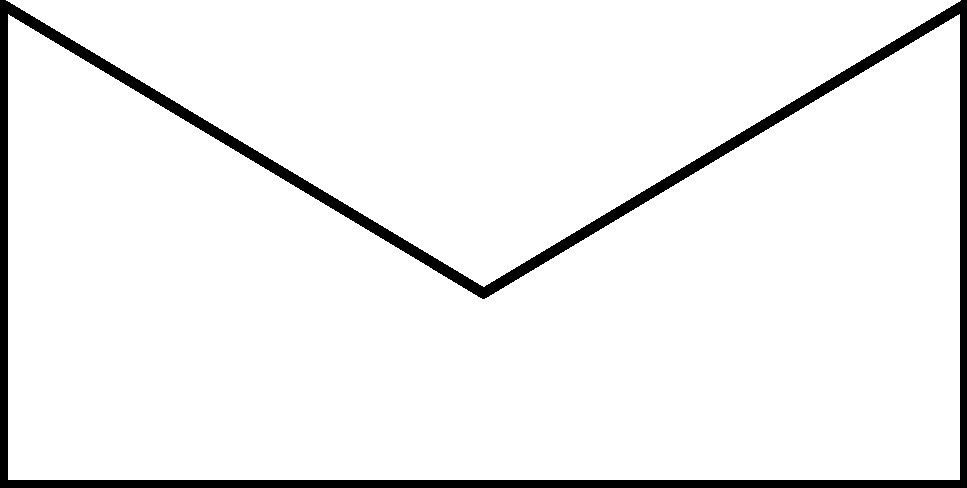
\includegraphics[width=\figheight,rotate=-90]{sources/method/overview/2D/input.pdf}
\caption{Layer outline}\label{overview_outline}
\end{subfigure}
\begin{subfigure}{\figwidth}\centering
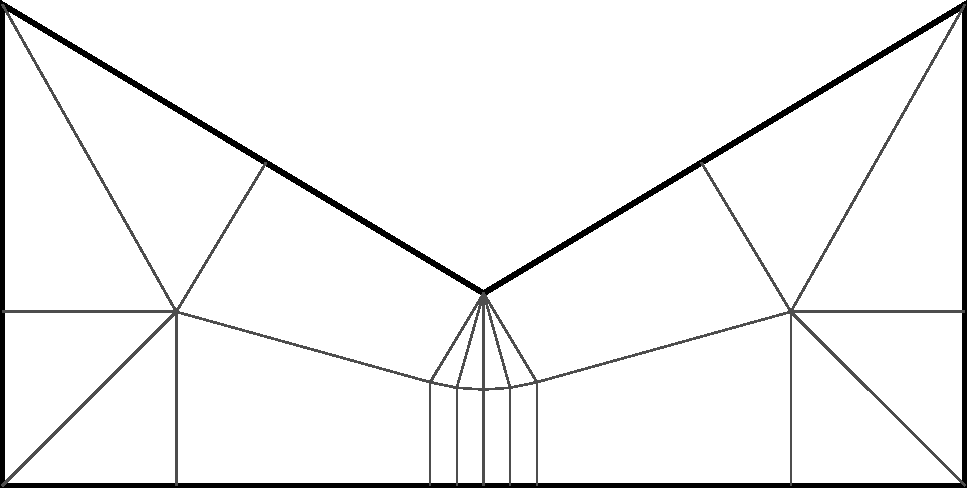
\includegraphics[width=\figheight,rotate=-90]{sources/method/overview/2D/uoc.pdf}
\caption{Skeleton}\label{overview_skeleton}
\end{subfigure}
\begin{subfigure}{\figwidthTwo}\centering
\hspace*{\tempheightTwo}
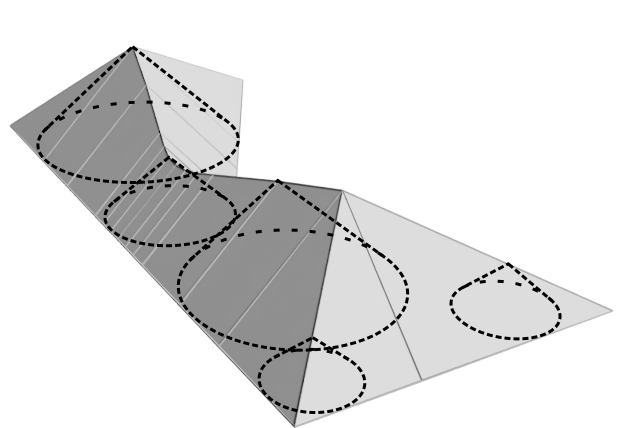
\includegraphics[height=\figheight]{sources/method/overview/surface/UoC_with_cones.png}
\caption{Union of cones}\label{overview_uoc}
\end{subfigure}
\begin{subfigure}{\figwidthTwo}\centering
\hspace*{\tempheightTwo}
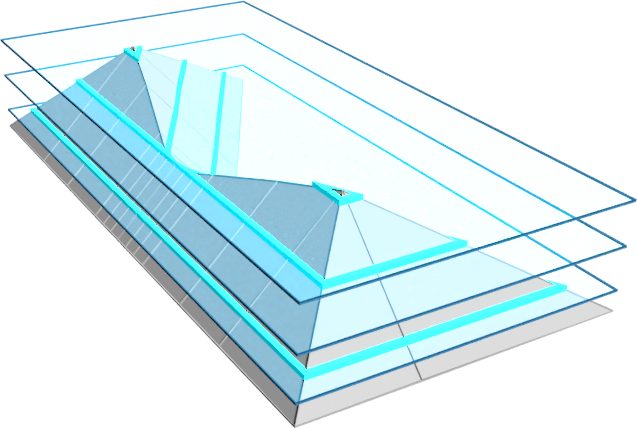
\includegraphics[height=\figheight]{sources/method/overview/surface/sliced_naive_cropped.png}
\caption{Slicing}\label{overview_uniform_sliced}
\end{subfigure}
\begin{subfigure}{\figwidth}\centering
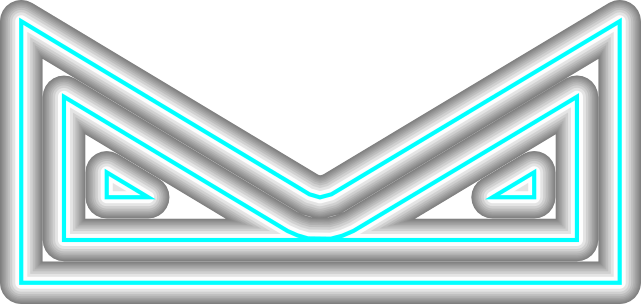
\includegraphics[width=\figheight,rotate=-90]{sources/method/overview/2D/naive.png}
\caption{Uniform paths}\label{overview_uniform_paths}
\end{subfigure}


\setlength{\figwidth}{.22\textwidth}
\setlength{\figwidthTwo}{.17\textwidth}
\setlength{\figwidthTree}{.22\textwidth}
\setlength{\tempheight}{-0.3cm}
\setlength{\tempheightTwo}{-0.5cm}
\begin{subfigure}{\figwidth}\centering
\hspace*{\tempheightTwo}
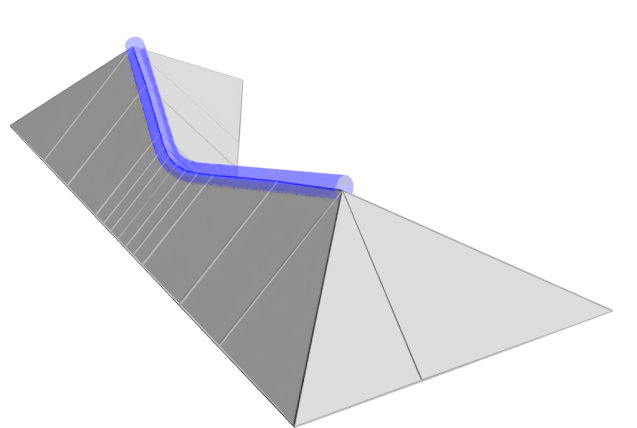
\includegraphics[height=\figheight]{sources/method/overview/surface/marking_cropped.png}

\vspace{\tempheight}

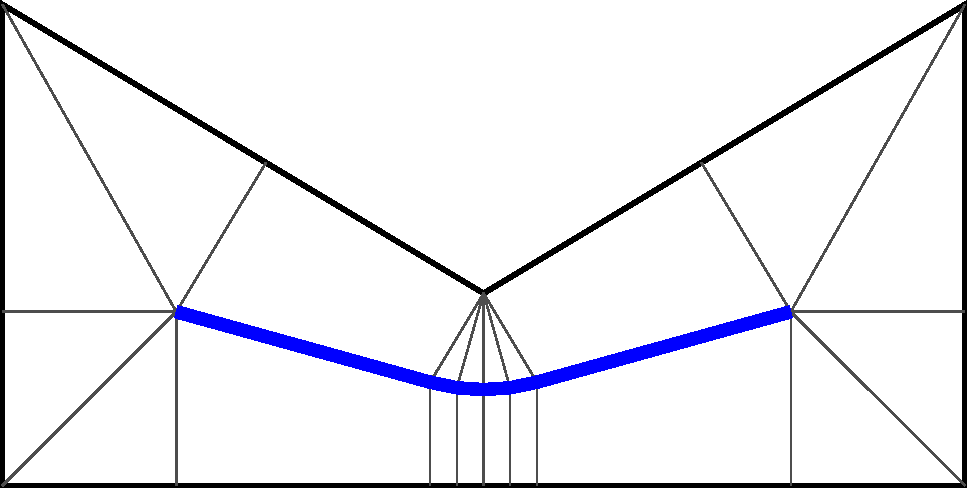
\includegraphics[width=\figheight]{sources/method/overview/2D/marked.pdf}
\caption{Center identification}\label{3d_surface_overview_center}
\end{subfigure}
\begin{subfigure}{\figwidth}\centering
\hspace*{\tempheightTwo}
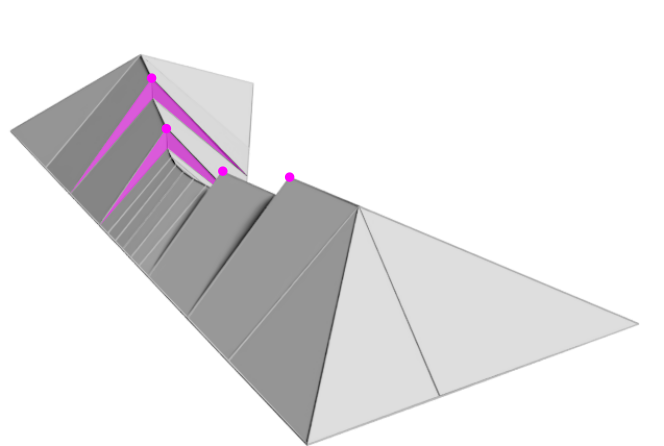
\includegraphics[height=\figheight]{sources/method/overview/surface/quantized.png}

\vspace{\tempheight}

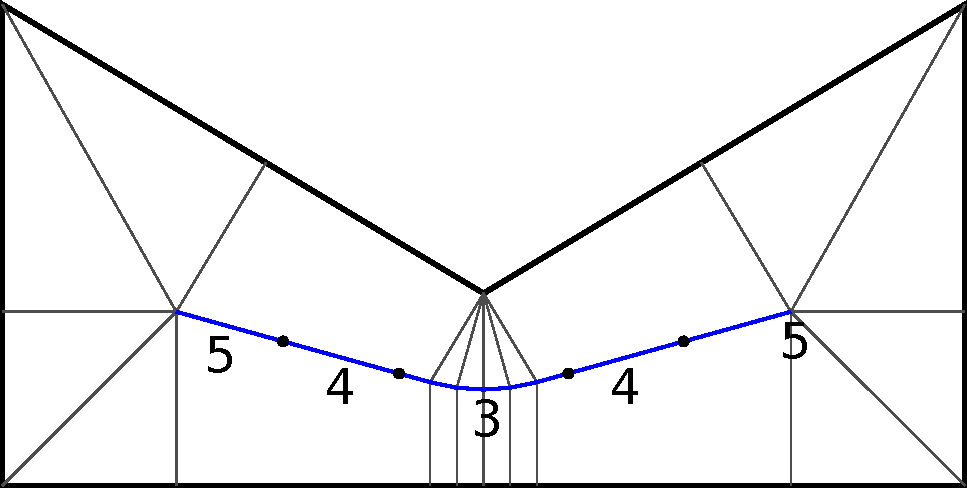
\includegraphics[width=\figheight]{sources/method/overview/2D/rounded.pdf}
\caption{Quantization}\label{3d_surface_overview_rounded}
\end{subfigure}
\begin{subfigure}{\figwidth}\centering
\hspace*{\tempheightTwo}
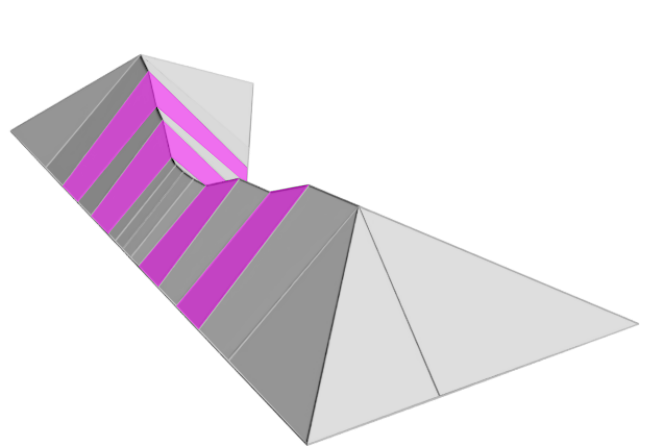
\includegraphics[height=\figheight]{sources/method/overview/surface/smoothed_magenta.png}

\vspace{\tempheight}

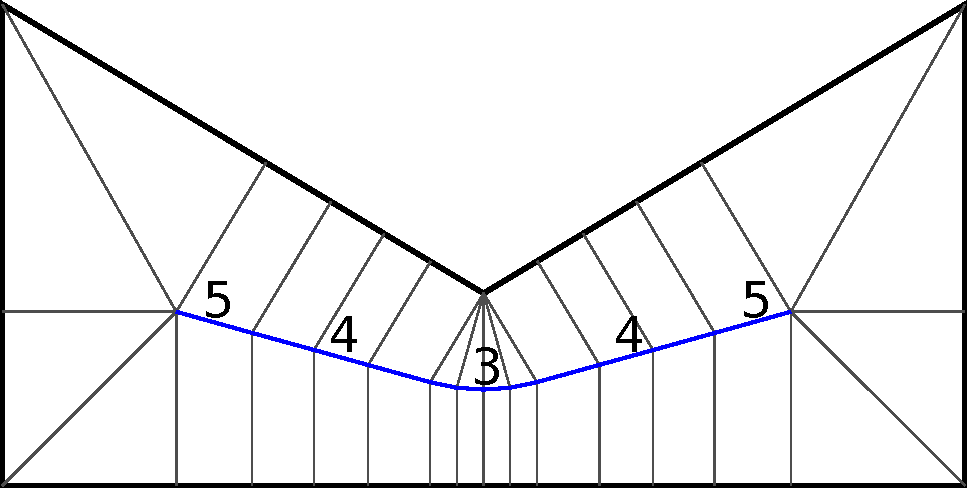
\includegraphics[width=\figheight]{sources/method/overview/2D/smoothed.pdf}
\caption{Smoothing}\label{3d_surface_overview_smoothed}
\end{subfigure}
\begin{subfigure}{\figwidth}\centering
\hspace*{\tempheightTwo}
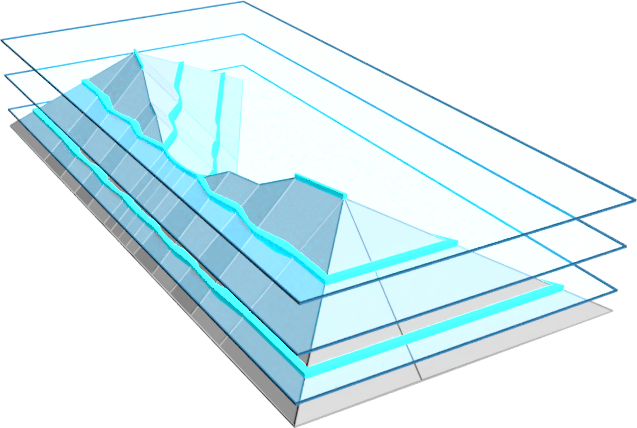
\includegraphics[height=\figheight]{sources/method/overview/surface/sliced_cropped.png}

\vspace{\tempheight}


\includegraphics[width=\figheight]{sources/method/overview/2D/sliced.png}
\caption{Adaptive width paths}\label{3d_surface_overview_sliced}
\end{subfigure}
\caption{
The first row illustrates the generation of uniform paths \subref{overview_uniform_paths}
by interpreting the path as the intersection between horizontal planes and the union of cones \subref{overview_uoc}, which is an alternative visualization of the skeleton \subref{overview_skeleton}. 
The second row depicts the stages with both 2D and 3D visualizations for generating paths with adaptive width \subref{3d_surface_overview_sliced}.
Central elements in the skeleton are first identified (blue in \subref{3d_surface_overview_center}).
The heights are then quantized in terms of number of beads (the integer values in \subref{3d_surface_overview_rounded}), and smoothed \subref{3d_surface_overview_smoothed}.
}
\label{3d_surface_overview}
\end{figure*}

For ease of reference we have included a legend showing the terms employed in this manuscript in \cref{legend}.
These terms will be further explained as they first appear later in this paper. 

\begin{figure}\centering
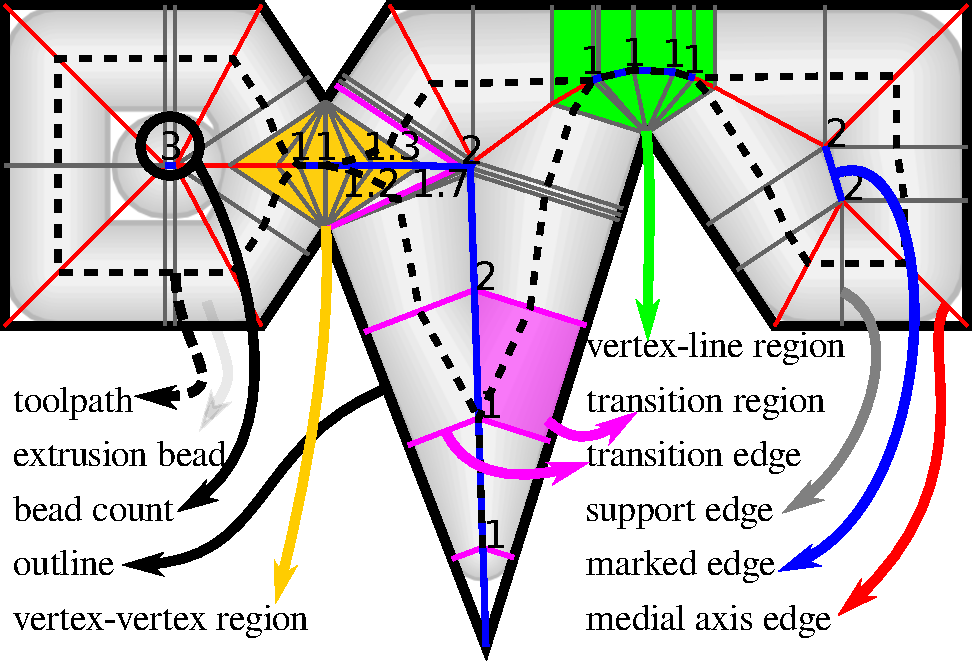
\includegraphics[width=.75\columnwidth]{sources/method/legend2.pdf}
\caption{Illustrative explanation of terms and color coding that are consistently used in this paper.}
\label{legend}
\end{figure}




















%\subsection{Surface generation}\label{sec_surface_construction}
\subsection{Union of cones}\label{sec_surface_construction}

The union of cones (UoC) is derived from a common skeletonization of the polygonal outline shape: the medial axis.
By assigning each node in the skeleton a height equal to its shortest distance to the outline we obtain the shape of the UoC.
Starting from the medial axis we further decompose the shape into simple fragments, so that the domain contains only quads and triangles.
This decomposition constitutes an approximation of the UoC. 


%\subsubsection{Medial axis transform}
\paragraph{Medial axis transform}
The medial axis is a compact and complete representation of a shape.
It is defined as the set of positions where the inscribed circle meets the boundary in at least two locations~\cite{blum1967transformation,lee1982medial}.
The resulting skeleton consists of straight edges and parabolic edges.
An example is illustrated in \cref{shape_decomposition_mat}.
We call the set of points on the outline polygon $P$ closest to a skeletal point $v$ its \emph{support}:
\begin{equation}
    \text{sup}(v) = \argmin_{x\in P} |x - v|.
\end{equation}
The shortest distance for a point on the skeleton is called its feature radius, $R(v)$.
%See \cref{MAT_explanation_circles}.
%We therefore represent the skeleton in a standard half-edge data-structure.
%See \cref{shape_decomposition_datastructure}.
%Alternatively the medial axis can be defined as the locations where the UoC surface is discontinuous \cite{blum1967transformation}
%The medial axis can therefore be seen as the space within which contour following toolpaths are generated.
%See \cref{MAT_explanation}.
The medial axis along with the feature radius values along the skeleton form a complete shape descriptor, known as the medial axis transform (MAT).
%Feature radius and node locations will be used below to analyse the shape locally.

By vertically raising the center of an inscribed circle to a height that equals the center's feature radius, a cone is formed. 
The union of all such cones forms a 3D solid volume. 
The medial axis can thus also be interpreted as ribs of the surface of the union of cones.~\cite{blum1967transformation}



\begin{figure}\centering
\setlength{\figwidth}{0.24\columnwidth}
\setlength{\figwidthTwo}{0.3\columnwidth}
\begin{subfigure}[t]{\figwidth}\centering
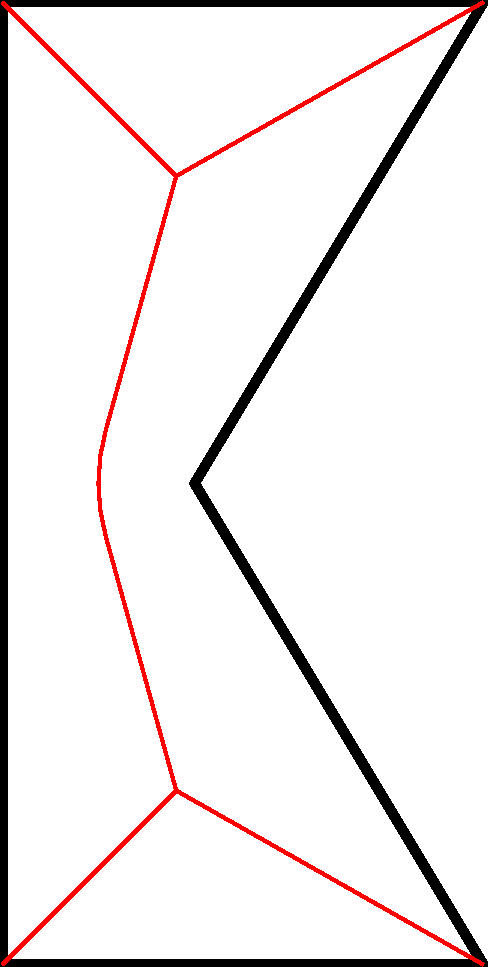
\includegraphics[height=\figwidthTwo]{sources/method/simple_skeleton_mat}
\caption{Medial Axis}\label{shape_decomposition_mat}
\end{subfigure}
\begin{subfigure}[t]{\figwidth}\centering
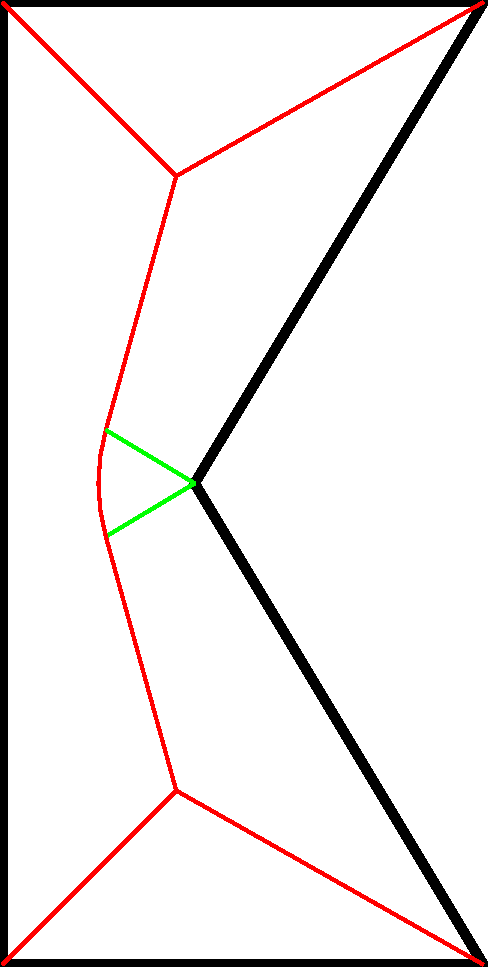
\includegraphics[height=\figwidthTwo]{sources/method/simple_skeleton_vd}
\caption{Voronoi Diagram}\label{shape_decomposition_vd}
\end{subfigure}
\begin{subfigure}[t]{\figwidth}\centering
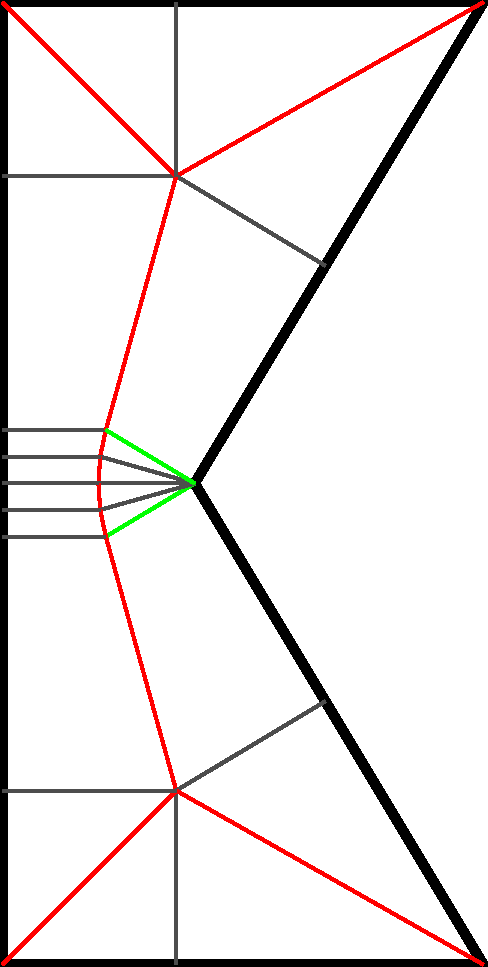
\includegraphics[height=\figwidthTwo]{sources/method/simple_skeleton_st}
\caption{Skeletal Trapezoids}\label{shape_decomposition_st}
\end{subfigure}
\begin{subfigure}[t]{\figwidth}\centering
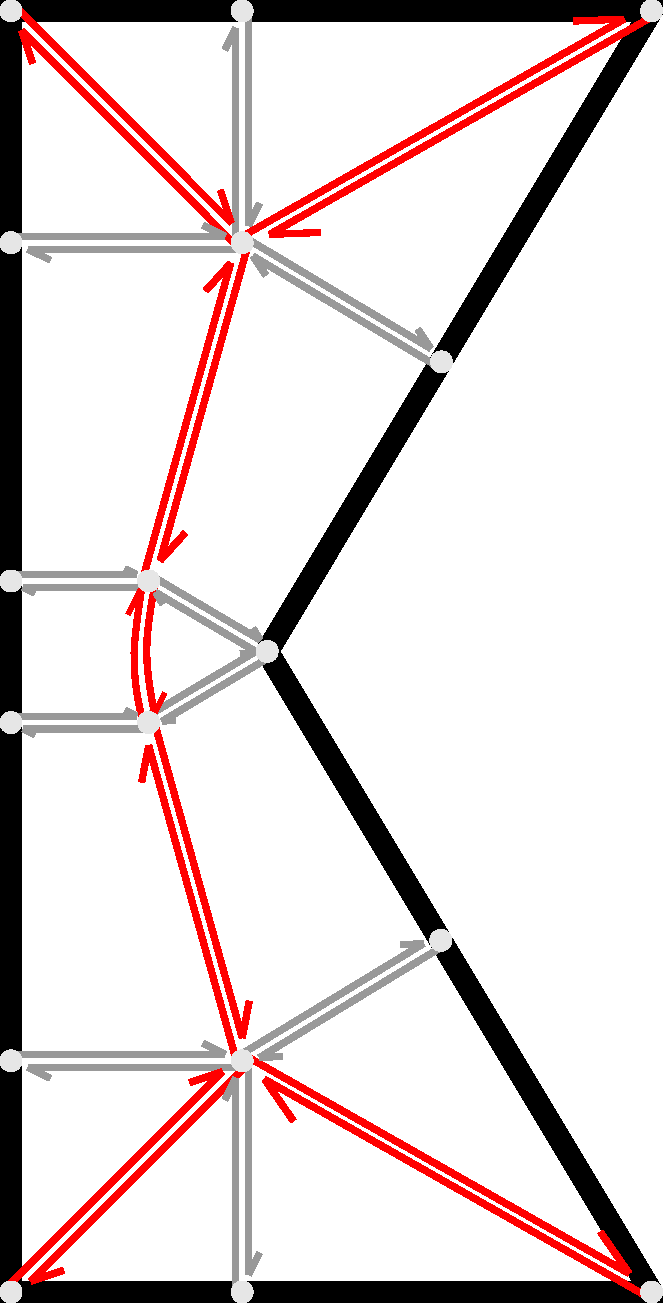
\includegraphics[height=\figwidthTwo]{sources/method/half_edge_datastructure.pdf}
\caption{Data structure}\label{shape_decomposition_datastructure}
\end{subfigure}
\caption{
Skeletonization of an outline shape (black).
Relation between the medial axis (red), the limited Voronoi Diagram (red and green) and the Skeletal Trapezoidation (red, green and gray): MAT $\subset$ Limited VD $\subset$ ST.
\subref{shape_decomposition_datastructure} We can represent a skeleton using a half-edge data-structure.
}
\label{skeletonization_comparison}
\end{figure}



%\subsubsection{Skeletal trapezoidation}
\paragraph{Skeletal trapezoidation}
Starting from the medial axis we decompose the input polygon into a set of quads and triangles, so that we can perform the slicing stage on simple shapes.
We employ a shape decomposition similar to the one proposed by \citeauthor{Ding2016a}~\cite{Ding2016a}. 
The basic idea is to add edges connecting each node $v$ on the medial axis to (all of) its supports, $\text{sup}(v)$. 
The resulting skeleton decomposes the outline shape into trapezoids and triangles.
Considering the fact that the concept of trapezoidation conventionally allows for the degenerate case where a trapezoid resolves into a triangle~\cite{chazelle1984,fournier1984}, we call this shape decomposition the \emph{Skeletal Trapezoidation} (ST).


The edges generated from MAT can be classified into three types: (a) line-line edge -- straight edge generated from two line segments in the outline polygons, (b) vertex-line edge -- parabolic edge resulting from an outline vertex and a line segment in the outline, and (c) vertex-vertex edge -- straight edge resulting from two outline vertices.
The vertex-line and vertex-vertex edges are discretized into pieces with a length up to $d^\text{discretization}$.
This allows to approximate the feature radius in between two discretized nodes $v_0$ and $v_1$ by linear interpolation. 
Again we connect the newly inserted nodes to their support, which results in vertex-line regions and vertex-vertex regions such as depicted in \cref{legend}.


% The ST contains all edges from the medial axis which are generated from two line segments in the outline polygons.
% The interaction between an outline vertex and a line segment results in a parabolic edge, which is discretized into pieces with a length up to $d^\text{discretization}$ (see the middle of \cref{shape_decomposition_st}).
% Additionally medial axis edges which are generated from two outline vertices are also discretized, so that the feature radius $R$ in between two discretized nodes $v_0$ and $v_1$ can be approximated by linear interpolation between $R(v_0)$ and $R(v_1)$.
% Again we connect the nodes which are introduced by the discretization to their support, which results in vertex-line regions and vertex-vertex regions such as depicted in \cref{legend}.



%\subsubsection{Union of cones}
\paragraph{Approximation of union of cones}
The skeleton trapezoidation (ST) provides a means to visualize the union of cones (UoC) approximated by a 3D surface mesh composed of quadrilateral and triangular patches.
%In order to visualize the ST as a 3D surface, we add a third dimension.
We assign each node in ST a (real number) height value measured in terms of beads, referred to as the \emph{bead count} $b$.
We define the bead count as the number of beads to fit along the \emph{diameter} of the inscribed circle centered at node $v$, i.e. $2R(v)$, by
\begin{equation}
    b^\sim_v = 2 R(v) / w^*,
\label{eq:initialBeadCount}
\end{equation}
where $w^*$ is the nozzle size. 
%While the feature radii are measured along the support edges, the diameter is not measurable as such because the support edges are generally not collinear;
We divide the diameter rather than the radius as this allows to deal with an odd number of beads while using integer logic.
%The result is a mesh representing the union of cones (UoC) consisting entirely of quads and triangles.
Note that although the overview of the method has been described geometrically in terms of the UoC, the actual toolpath generation relies on the two-dimensional ST, while the use of the bead count as a height value is only a visualization aid.







\paragraph{Implementation}
The medial axis of a polygonal shape is a subset of the Voronoi Diagram generated from the line segments and vertices of the shape~\cite{lee1982medial}. 
The edges of the Voronoi diagram that fall outside of the outline shape are irrelevant for our purpose and thus discarded.
Note that the Voronoi diagram contains, in addition to the medial axis, edges connecting to concave vertices in the outline shape (see \cref{shape_decomposition_vd}). 
These extra edges are a subset of the edges connecting a node to its support, so we keep them in.
From the Voronoi diagram we add nodes to discretize parabolic edges and edges formed by two concave outline vertices, and then connect all nodes to their supports, forming a skeletal trapezoidation. 
We then assign each node the bead count values using \cref{eq:initialBeadCount}.
We compute the Voronoi diagram using the Boost \verb!C++! libraries~\cite{schaling2011boost}, which implements the algorithm proposed by \citeauthor{fortune1986sascg}~\cite{fortune1986sascg}.
A half-edge data-structure is used to represent the Voronoi diagram (\cref{shape_decomposition_datastructure}).

%









\subsection{Center classification}\label{sec_center_classification}
%The simple technique of performing uniform width offset produces large overfill and underfill areas on central regions of the ST.
%These central regions present themselves as upper ridges in the mountains of the UoC surface.
%In order to prevent the over- and underfill we will change the bead counts in the central regions.
%This sections covers what parts of the UoC will be marked as being central.
In order to prevent over- and underfill to occur in central, we mark parts of the UoC \jun{ST?} as being central.
The remaining is called peripheral.
Our framework will decide on a beading at all of the marked nodes in `the center' and apply the beading outward to the unmarked nodes (\cref{sec_peripheral_height_adjustment}).

We mark a node in the ST as central if its feature radius is larger than that of all its neighboring nodes, i.e. a local maxima.
%That is: we mark the local maxima, i.e. the mountain tops of the UoC as being central.
We also mark an edge as being central if it is significant according to a significance measure.

%\subsubsection{Significance measure}\label{sec:significance_measure}
\paragraph{Significance measure}
We make use of the \emph{bisector angle} as an indicator of significance which is commonly used in shape analysis.
%Centrality can be formalized by looking at a commonly used significance measure knows as the \emph{bisector angle}.
The bisector angle $\alpha$ is the interior angle $\angle{p_0lp_1} \leq \SI{180}{\degree}$, between any location $l$ on an edge of the ST and its two supporting points $ \{ p_0, p_1 \} = \text{sup}(l)$~\cite{attali1996modeling}. 
An edge is significant if the bisector angle on any location on the edge exceeds a prescribed $\alpha_\text{max}$. 
As illustrated in See \cref{naive_overfill_underfill}, for a polygon with a pointy wedge area of an angle $\beta$, we have $\alpha = 180\degree - \beta$. This corresponds to overfill areas and underfill areas the size of $\nicefrac12 (w^*)^2 \left( \nicefrac14 \tan ( \alpha / 2) - \alpha / 2 \right)$ when filled using the simple technique of uniform bead width $w^*$.
The bisector angle is therefore an exact indicator of the amount of overfill and underfill in the uniform toolpaths of constant width.
%Contrary to related literature we will \emph{keep} the non-significant regions of the skeleton.
%We mark all significant edges as such and contrary to related literature we keep the unmarked edges of the ST.


\begin{figure}
\centering
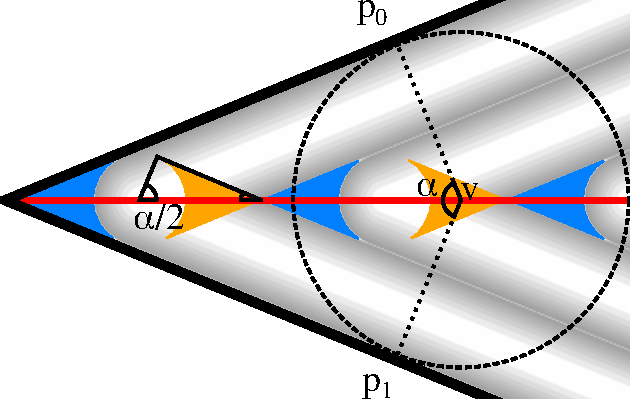
\includegraphics[width=.5\columnwidth]{sources/method/naive_overfill_underfill.pdf}
\caption{
Overfill and underfill areas in a simple toolpathing using a uniform bead width $w$ for a wedge area with vertex angle $\beta$.
The underfill areas (light blue) are mirrored versions of the overfill areas (dark red).
The bisector angle $a = 180\degree - \beta$ is the angle between a location $v$ and its support $p_0$ and $p_1$.
}
\label{naive_overfill_underfill}
\end{figure}

% The significance evaluation is performed efficiently by checking the ratio between feature radius $R$ and the Euclidean distance:
% if $ | R(v_1) - R(v_0) | / |v_1 - v_0| >  \cos(\alpha_\text{max} / 2)$ then $\alpha > \alpha_\text{max}$. See \cref{distance_based_angles}. This ratio has a clear geometrical interpretation as the slope of the ridge in the UoC surface.

To avoid evaluating the bisection angle at any location on all edges, we devise an efficient measure which operates only on the two nodes of an edge.
Because all locations along a line-line edge have the same bisector angle we can evaluate whether the edge is significant by checking whether 
\begin{align}\label{simple_significance_measure}
| R(v_1) - R(v_0) | / |v_1 - v_0| >  \cos(\alpha_\text{max} / 2)
\end{align}
(see \cref{distance_based_angles}).
This ratio has a clear geometrical interpretation as the slope of the ridge in the UoC surface.
For vertex-line edges and vertex-vertex edges only a portion of the edge may be significant.
We therefore introduce nodes at the boundaries of the significant portion during the discretization of such edges (see Appendix \cref{edge_discretization}).
The significance of all edges can then accurately be evaluated using \cref{simple_significance_measure}.

\begin{figure} \centering
\newlength{\significancePropertiesHeight}
\setlength{\significancePropertiesHeight}{.25\columnwidth}
\begin{subfigure}{0.35\columnwidth} \centering
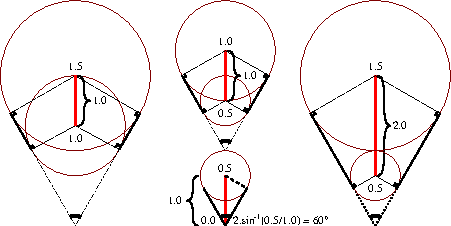
\includegraphics[height=\significancePropertiesHeight]{sources/method/distance_based_angles.pdf}
\caption{Significance}
\label{distance_based_angles}
\end{subfigure}
\begin{subfigure}{0.3\columnwidth} \centering
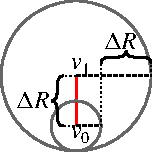
\includegraphics[height=\significancePropertiesHeight]{sources/method/distance_ratio_limit.pdf}
\caption{Distance}
\label{distance_ratio_limit}
\end{subfigure}
\begin{subfigure}{0.3\columnwidth} \centering
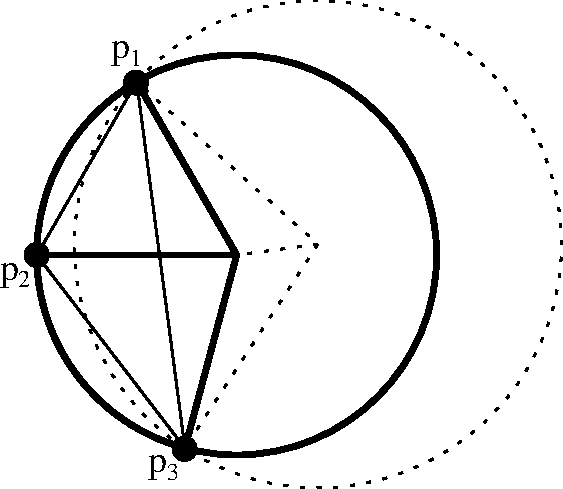
\includegraphics[height=\significancePropertiesHeight]{sources/method/branch_upward_edge_property.pdf}
\caption{Upward edge}
\label{branch_upward_edge_property}
\end{subfigure}
\caption{
Properties of feature radius $R$.
Part of outline shape in thick black,
ST edges in red,
inscribed circle in gray,
radii in dashed lines.
\subref{distance_based_angles} The significance measure can be simplified using $\alpha = 2 \gamma = 2 \cos^{-1} \Delta R / |v_1 - v_0|$.
\subref{distance_ratio_limit} The distance $|v_1 - v_0| > \Delta R$ because otherwise the feature radius would not be one of an inscribed circle.
\subref{branch_upward_edge_property} The radial distance can only increase along one edge around a branch point in the medial axis.
}
\end{figure}





%\subsubsection{Marking filtering}
\paragraph{Marking filtering}
After initializing the marking at all edges and nodes, we filter out high frequency changes in the marking in order to ensure that the generated toolpath is smooth. 
The filtering is performed by additionally marking some unmarked elements, rather than the opposite since unmarking central regions reintroduce large over- and underfill areas.
From each marked node $v_0$ with an upward unmarked edge attached we walk along the upward edges;
if the total length traversed until we reach another marked node $v_1$ is shorter than some filter distance $d_\text{max}^\text{unmarked}$, we mark all edges encountered as being central.















\subsection{Central height adjustment}\label{sec_central_height_adjustment}
Now that we have identified and marked the central regions we quantize their heights.
We first quantize the initial bead count $b^\sim$ into an integer bead count $b^\neg$ at the marked nodes using a quantization operator $q$,
then find the locations along the edges where $q$ makes a jump from one bead count $n$ to another $n+1$
and then introduce ramps to smoothly transition from $n$ to $n+1$ using fractional bead counts $b^\wedge$ along the smooth transition.
%\subsubsection{Initial bead count}\label{sec_initial_bead_count}



\begin{figure*}
\centering
\setlength{\figwidth}{0.13\textwidth}
\begin{subfigure}{\figwidth}
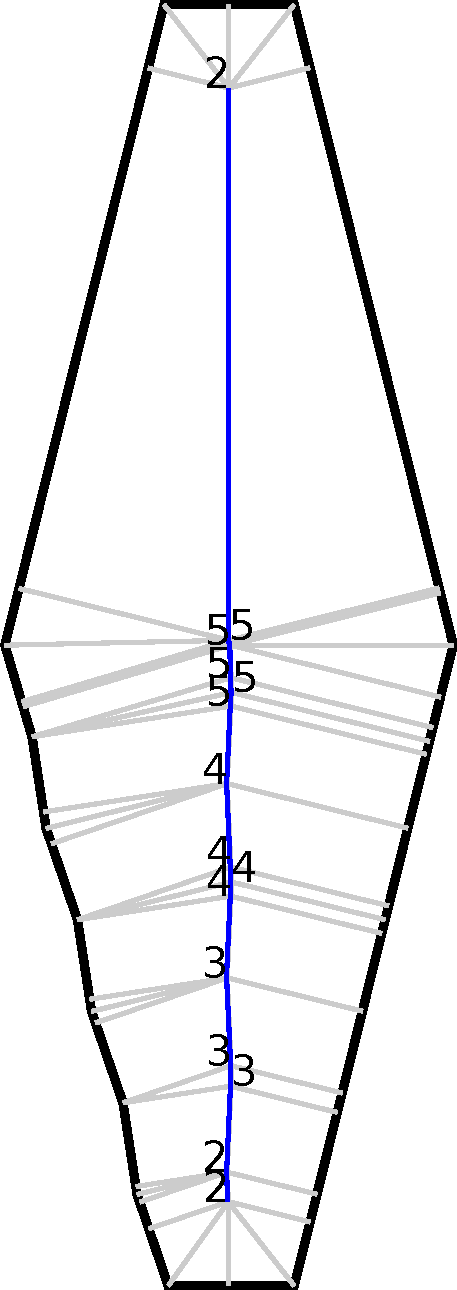
\includegraphics[width=\columnwidth]{sources/method/beading_transitioning_filtering__bead_count.pdf}
\caption{Quantized bead counts}\label{beading_transitioning_filtering__bead_count}
\end{subfigure}
\begin{subfigure}{\figwidth}
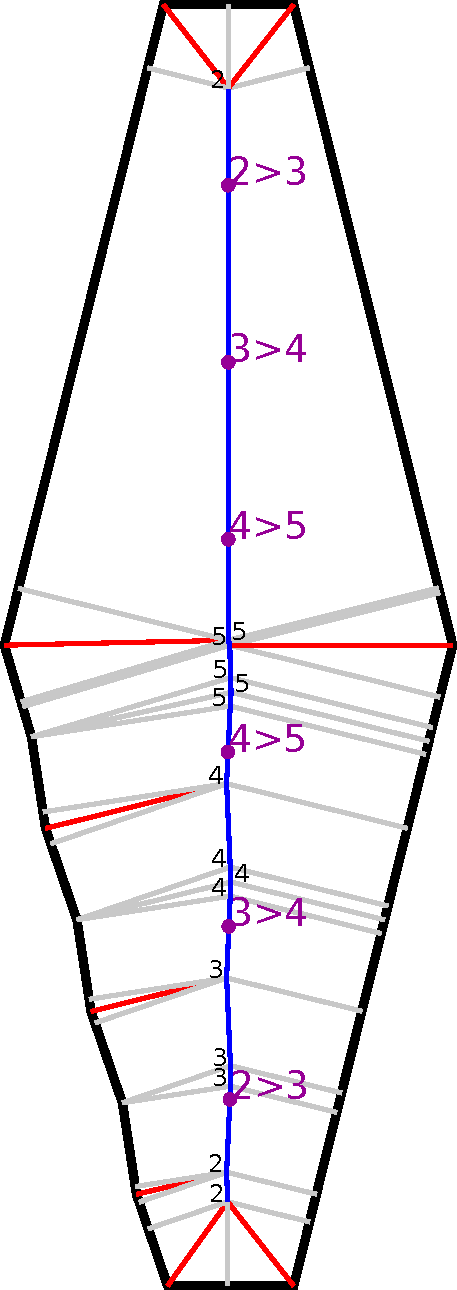
\includegraphics[width=\columnwidth]{sources/method/beading_transitioning_filtering__transition_mids.pdf}
\caption{Transition anchors}\label{beading_transitioning_filtering__transition_mids}
\end{subfigure}
\begin{subfigure}{\figwidth}
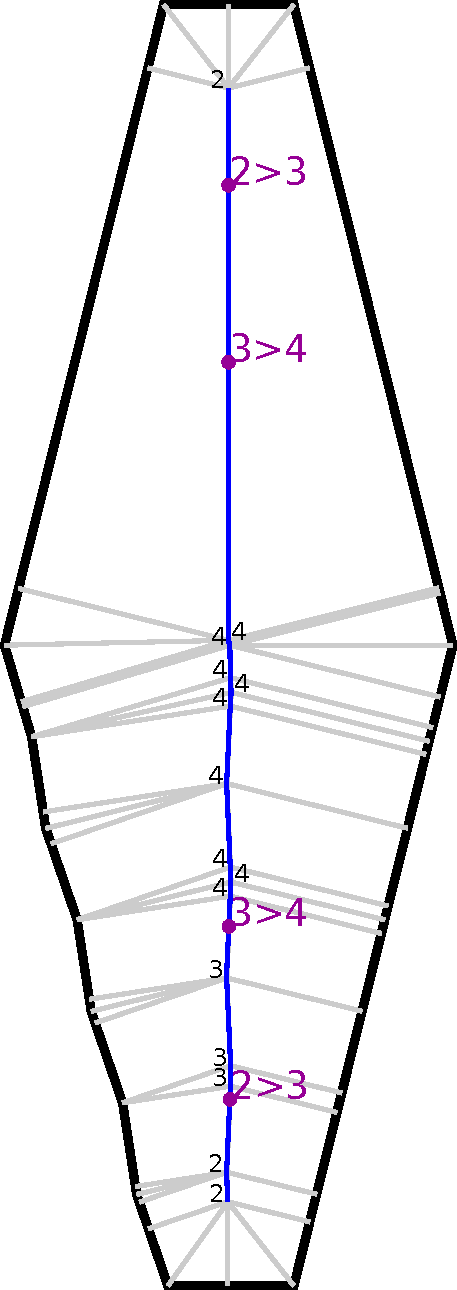
\includegraphics[width=\columnwidth]{sources/method/beading_transitioning_filtering__filtered.pdf}
\caption{Filtered anchors}\label{beading_transitioning_filtering__filtered}
\end{subfigure}
\begin{subfigure}{\figwidth}
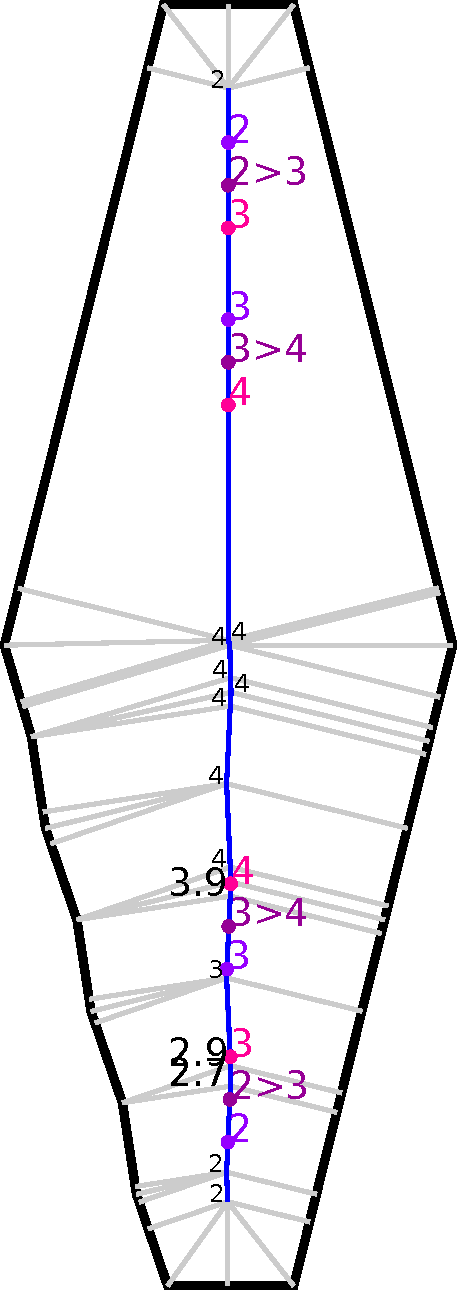
\includegraphics[width=\columnwidth]{sources/method/beading_transitioning_filtering__transition_ends.pdf}
\caption{Transition ramp ends}\label{beading_transitioning_filtering__transition_ends}
\end{subfigure}
\begin{subfigure}{\figwidth}
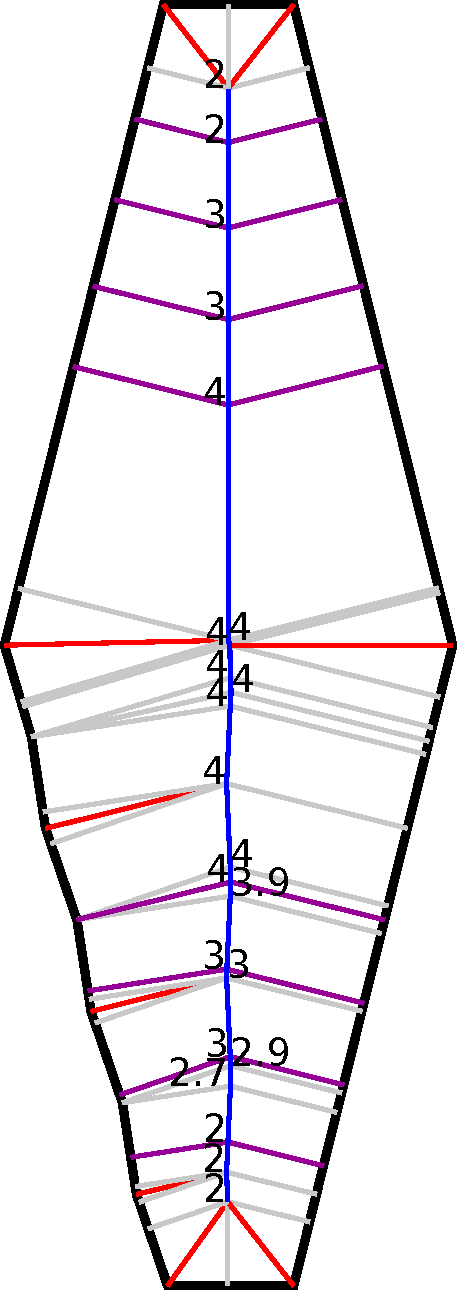
\includegraphics[width=\columnwidth]{sources/method/beading_transitioning_filtering__transitions_applied.pdf}
\caption{Radial support edges}\label{beading_transitioning_filtering__transitions_applied}
\end{subfigure}
\begin{subfigure}{.27\textwidth}
\hspace*{-.5cm}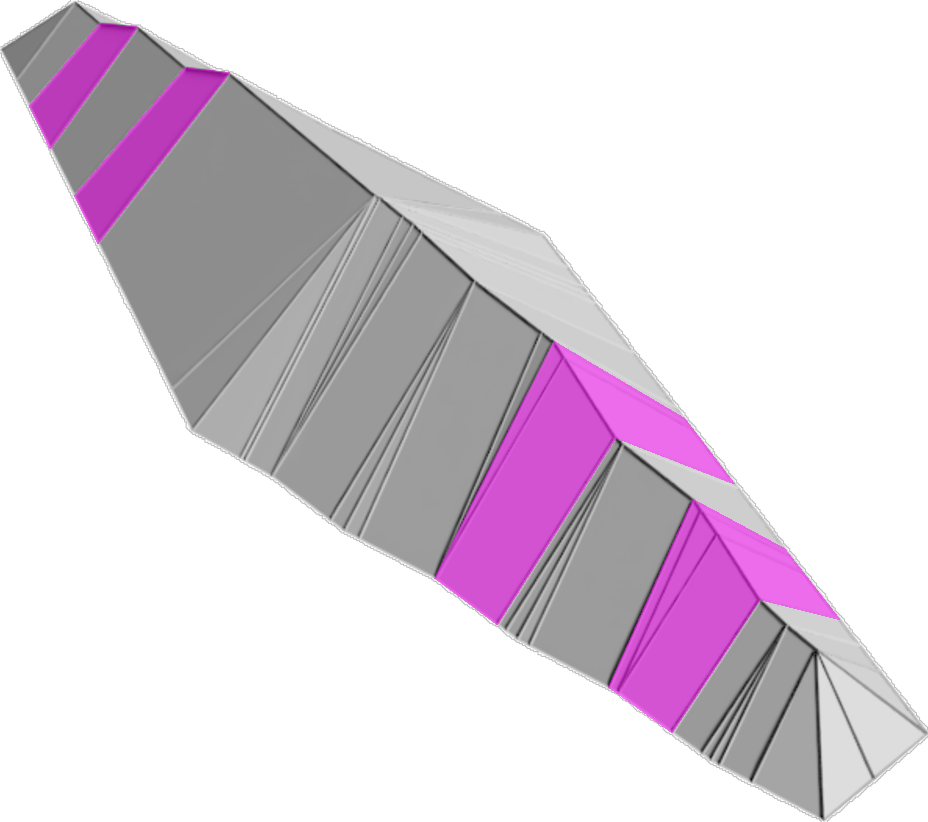
\includegraphics[width=1.2\columnwidth]{sources/method/beading_transitioning_filtering__result_uoc.pdf}
\caption{Result UoC}\label{beading_transitioning_filtering__result_uoc}
\end{subfigure}
\caption{
Applying bead counts and transitioning on a shape showing the difference between a simple ST (top) and a mirrored version with small perturbations in the outline (bottom).
Outline in black, medial axis edges in red, radial edges in grey.
\subref{beading_transitioning_filtering__bead_count} First we initialize the bead counts (black) in the marked regions (blue).
\subref{beading_transitioning_filtering__transition_mids} We then extract the anchor locations (purple) of the transitions to a different bead count should be.
\subref{beading_transitioning_filtering__filtered} We then filter out regions of constant bead count.
\subref{beading_transitioning_filtering__transition_ends} We then calculate the end locations (magenta, pink) of the transitions and modify the bead count at nodes in between to fractional values.
\subref{beading_transitioning_filtering__transitions_applied} Finally we introduce nodes at the ends and introduce radial edges (purple) as per the trapezoidation constraint.
The symmetry in the result shows that transitioning is robust against small perturbations in the outline shape.
}
\label{beading_transitioning_filtering}
\end{figure*}


%\subsubsection{Quantization}

\paragraph{Quantization}
We define a quantization operator $q$ to map a feature diameter ($d=2R(v)$) to a bead count: $q: \mathbb{R} \to \mathbb{N}$.
Because our quantization scheme should round to the nearest integer multiple of the nozzle size, we have
$q(d) = \left\lfloor d / w^* + \nicefrac12 \right\rfloor$.
Alternative quantization schemes will be discussed in \cref{sec_generalization}.
By applying $q$ to the heights of central nodes we quantize the bead count:
$b^\neg_v = q(2R(v)) = \left\lfloor b^\sim_v + \nicefrac12 \right\rfloor$.
\iffalse
Along with this quantization, an amendment to the marking filtering is performed, in order to alleviate a problem that will be handled in \cref{section_beading_conflicts}.
Specifically, unmarked regions are marked as central if they lie between two nodes with the same integer bead count.
\fi
%We then filter out short unmarked regions where the bead count remains constant in order to limit the extent of a problem handled in \cref{section_beading_conflicts}.
% From each marked node $v_0$ with an upward unmarked edge attached we walk along the upward edges until we hit another marked node $v_1$.
% If the upper node has the same bead count $b^*_{v_1} = b^*_{v_0}$ we mark all edges and nodes $v$ in between, and set the bead count $b^*_v \leftarrow b^*_{v_0}$.

\paragraph{Transition anchors}
For a marked edge which connects nodes $v_0$ and $v_1$ with $b^\neg_{v_0} \le n < b^\neg_{v_1}$, we determine the \emph{transition anchor locations} at which the bead count transitions from $n$ to $n+1$.
To this end, we introduce the function 
\begin{equation}
    q^{-1}(n) := \argmax_d q(d) = n,
\end{equation}
which gives the feature diameter $d$ at which the bead count $q$ transitions from $n$ to $n+1$.
The location of the anchor $v_x$ is then computed by inversely interpolating $R(v_x) = q^{-1}(n)$, i.e. 
\begin{equation}
    v_x = v_0 + (v_1 - v_0) \frac{ q^{-1}(n) - R(v_0) }{ R(v_1) - R(v_0) }.
\end{equation}
%for each $n$ such that $b^*_{v_0}\le n<b^*_{v_1}$.
An illustration of the anchors is shown in \cref{beading_transitioning_filtering__transition_mids}.

We perform a filtering step to prevent frequently changing the bead count back and forth within a short distance.
For two consecutive anchors which transition to opposite directions, if the distance between them is smaller than some limit $d_\text{max}^\text{transition}$, the bead counts at all nodes in-between are set to the surrounding bead counts, and consequently these anchors are removed (See \cref{beading_transitioning_filtering__filtered}).

% For each edge which contains a transition anchor we walk along the marked edges until we encounter another anchor.
% If the other anchor is a transition in the opposite direction and the traversed distance is within some limit $d_\text{max}^\text{transition}$ we remove the transitions and set the bead counts at all nodes in the filtered region to the surrounding bead counts.
% See \cref{beading_transitioning_filtering__filtered}.






% \subsubsection{Smooth transition}
\paragraph{Smooth transitions}

A sharp transition from $n$ to $n+1$ beads at an anchor location creates sharp turns in the toolpath (see \cref{transitions} top).
A transition length $t(n)$ is introduced to ensure a smooth transition (see \cref{transitions}). 
The transition is centered at the anchor, and its length is set to $t(n) = w^*$.
We discard any transition anchor which is too close to the end of a chain of marked edges for the smoothed transition to fully fit within the marked region.
In order to make the transition ramps robust against small perturbations in the outline shape, we modify the nodes which are in between the two ends of the transition by (re-)assigning them a fractional bead count $b^\wedge$, linearly interpolated between the two ends of the transition (see \cref{beading_transitioning_filtering__transitions_applied}).
%This modification makes the transition ramps robust against small perturbations in the outline shape (to be explained in \cref{section_beading_interpolation});
%compare the top and bottom of \cref{beading_transitioning_filtering}. 
Finally we update the ST by adding support edges at the transition ends. 
As shown in \cref{beading_transitioning_filtering__result_uoc}, the marked regions in the UoC mesh have become horizontal at integer multiples of $\nicefrac12 w^*$ for long stretches with ramps in between.




\begin{figure}
\centering
\setlength{\figwidth}{\columnwidth}
\begin{subfigure}{0.9\figwidth}\centering
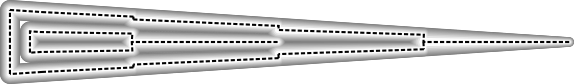
\includegraphics[width=\columnwidth]{sources/method/wedge_no_transitioning.png}
\caption{Without transitioning}
\end{subfigure}
\begin{subfigure}{0.9\figwidth}\centering
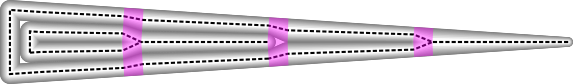
\includegraphics[width=\columnwidth]{sources/method/wedge_transitioning.png}
\caption{Transitioning}
\end{subfigure}
\caption{
Discontinuities around regions where the bead count changes are prevented by transition regions (highlighted in cyan).
}
\label{transitions}
\end{figure}














\subsection{Beading}\label{sec_peripheral_height_adjustment}

Now that we have transformed the heights in the central regions of the UoC we need to determine the heights in the rest of the shape, i.e. the periphery, and slice the resulting mesh into isocontour toolpaths.
The peripheral heights could be determined in a plethora of ways according to various beading schemes.
The ramps from the outline shape to the center might have various curves,
but for our example we use straight ramps, just like the original UoC.
See \cref{peripheral_heights}.
Mapping an original cone at apex $v$ to a cone with a height equal to the prescribed bead count $b$ of the central region is simply a matter of multiplying the $R$ values by $b / R(v)$.


\begin{figure}\centering
\setlength{\figheight}{.2\columnwidth}
\begin{subfigure}{.55\columnwidth}\centering
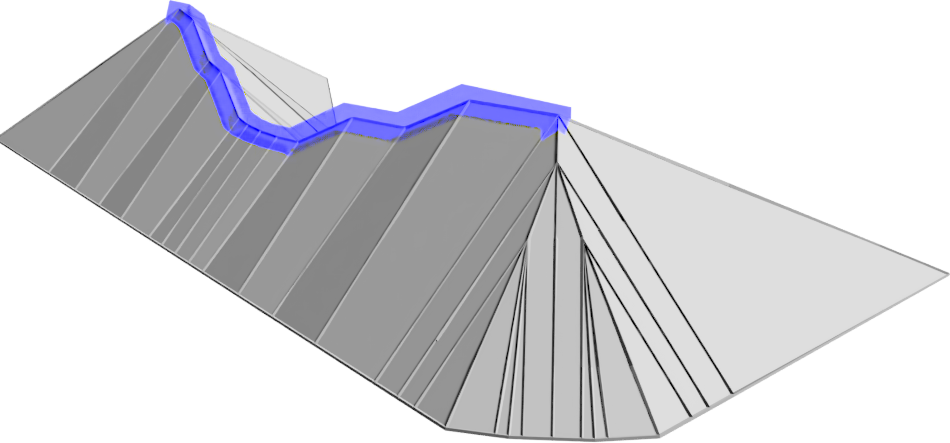
\includegraphics[height=\figheight]{sources/method/peripheral_heights_3D.png}
\caption{Surface mesh}
\end{subfigure}
\begin{subfigure}{.4\columnwidth}\centering
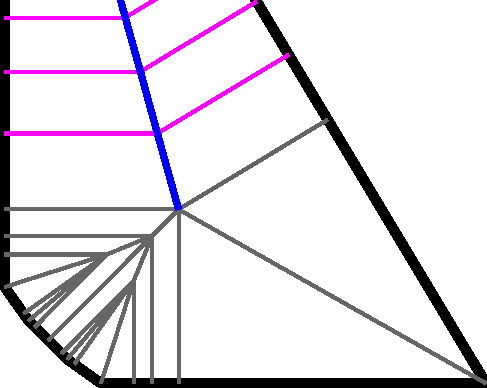
\includegraphics[height=\figheight]{sources/method/peripheral_heights.pdf}
\caption{ST}
\end{subfigure}
\caption{
Shallow corners will cause peripheral nodes for which the height should be determined based on the central node above it.
}
\label{peripheral_heights}
\end{figure}



However, for the purpose of generating toolpaths we only need to define the height at the locations which will be part of a slice, rather than at all locations in the periphery.
Instead of adjusting the height of peripheral mesh nodes, we determine the radial distances where the adjusted height coincides with a slicing height.
In this section we will show how we can define a mapping from radial distance values to the indices of slicing heights, called a \emph{beading},
how each beading is calculated for a central node
and how the beadings are propagated outward to peripheral nodes.
This helps to define an efficient slicing algorithm in \cref{sec_toolpath_extraction}.

\paragraph{Beading} 
We associate each central node $v$ with a set of radial distances for each bead along with the width of that bead, which we call the \emph{beading} $B$.
For our distributed beading scheme we define the beading for a central node $v$ with $n = b^\wedge_v$ beads and a diameter $d = 2R(v)$  as:
\begin{align*}
    %B &= \left\{ \left( w_0 , l_0 \right), \dots, \left( w_{n-1}, l_{n-1} \right) \right\} \\
    B(n,d) &= \left( \left\{  w_0 , \dots, w_{n-1} \right\}, \left\{ l_0 , \dots, l_{n-1} \right\} \right)\\
    w_i &= 2R(v) / n  & \text{for all $i \leq n$}\\
    l_i &= 2R(v) / n (i + \nicefrac12) & \text{for all $i \leq n$}
\end{align*}
where
$w_i$ and $l_i$ are the width and location of the $i$th bead,
respectively, counting from the outline inward.
An example beading is visualized in the top of \cref{beading_interpolation}:
$B^V$ cover the total horizontal distance $d$ using $n=4$ beads all with the same width and radial locations $l$ evenly divided over the length $d$.



\paragraph{Beading interpolation}
The beading is defined in terms of an integer number of beads, while we have assigned a fractional bead count to nodes within a transition region.
In order to generate a beading for a node $v$ with $n < b^*_v < n+1 $ we linearly interpolate the bead width and location of the first and last $n/2$ lines between a beading $B^V$ based on $n$ and a beading $B^W$ based on $n+1$ (see \cref{beading_interpolation}).
Such interpolation is also used to deal with beading conflicts (see \cref{beading_conflict_problem}).
We therefore also apply beading interpolation from a marked node $v_m$ upward along unmarked bones,
and interpolate between $v_m$ and the beading at the top of the slope over some distance $t_\text{beading}$ from the lower marked node.

\paragraph{Beading propagation}
The beading information is then broadcasted throughout the ST from central regions outward,
so that each unmarked node $v$ knows the beading of the marked node on top of the ramp on which $v$ is placed.
We first broadcast the beading information upward from all marked nodes,
so that we can then deal with beading conflicts in a downward phase.
This the downward phase makes sure that all nodes have a beading associated with it, so that the slicing algorithm can efficiently slice the edges leading up to a marked or unmarked node.	


\iffalse
The beading information will be used in the next phase to directly generate the sites of the toolpaths.
Note that a beading conceptually covers the whole diameter, while we only apply it along the radii;
the upper half of the beading is therefore unused.


% \subsubsection{Beading interpolation}\label{section_beading_interpolation}
\paragraph{Beading interpolation}
Central nodes which are in the middle of a transition have obtained a fractional bead count, but the definition of a beading presupposed integer numbers.
In order to generate a beading for a central node with a fractional bead count assigned we use the fractional part of the bead count to interpolate between two beadings defined on the fractional bead count rounded up and down.
Suppose we want to interpolate between two beadings $B^V$ and $B^W$, for which $n^{B^V} < n^{B^W}$.
We interpolate the diameter $d$, widths $w_i$ and locations $l_i$ for indices $i < \nicefrac12 n^{B^V}$ linearly and enforce the symmetry constraints on the upper indices.
See \cref{beading_interpolation}.
The linear interpolation enforces robustness against small perturbations in the outline shape which cause extra edges to appear in the ST inside of transition regions.

\iffalse
In order to create an interpolated beading $B = xB^V + (1-x) B^W$, for some $0<x<1$
we calculate:
\begin{align*}
n^{B} &= n^{B^W} \\
d^B &= x d^{B^V} + (1-x) d^{B^W} \\
w_i^{B} &= w_{n^B-i}^{B} = x w_i^{B^V} + (1-x) w_i^{B^W} \text{ for } i < \frac12 n^{B^V} \\
%  w_{frac{n}{2}^B - frac12}  = something difficult \text{ if } n \mod 2 == 1
w_i^{B} &= w_i^{B^W} \text{ otherwise}\\
l_i^{B} &= 
\begin{cases} 
x l_i^{B^V} + (1-x) l_i^{B^W} & \text{ for } i < \frac12 (n^{B^V} - 1) \\
d^B - x l_{i-n^{B^W}+n^{B^V}}^{B^V} + (1-x) l_i^{B^W} & \text{ for } i > n^B - 1 - \frac12 (n^{B^V} - 1) \\
\frac12 d^B  & \text{ if $n^B$ is odd and } i = (n^B - 1) / 2 \\
l_i^{B^W} - l_{n^{B^V}-1}^{B^W} + l_{n^{B^V}-1}^B & \text{ otherwise}
\end{cases}
\end{align*}
\fi

\begin{figure}
\centering
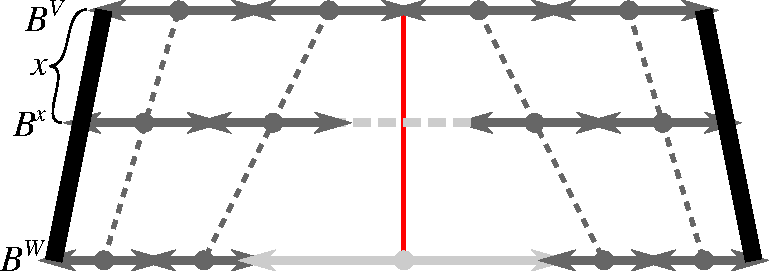
\includegraphics[width=.8\columnwidth]{sources/method/beading_interpolation_v2.pdf}
\caption{
Interpolation between two beadings $B^V$ and $B^W$ with a ratio $x$ results in a beading $B^x$.
Distances between the thick black lines constitute diameters $d$,
the toolpath locations are visualized as dots,
the widths are visualized as bidirectional arrows
and the middle is highlighted in red.
}
\label{beading_interpolation}
\end{figure}


% \subsubsection{Beading propagation}\label{section_beading_conflicts}
\paragraph{Beading propagation}
The beading information associated with the central nodes is then propagated outward throughout the whole mesh.
However, beading conflicts can arise where a marked edge has unmarked upward edges attached to them, since beading will also be propagated down from the local maxima or other higher marked regions.
See \cref{beading_conflict_problem}.
In such a case we interpolate between the lower beading and the beading propagated from above,
starting from the lower marked node and ending at a distance $t_\text{beading}$ upward.
At the nodes in between we will apply the interpolation between the two beadings and propagate the interpolated beading outward from those nodes.
This interpolation is performed during the beading propagation algorithm.

\fi

\begin{figure}\centering
\setlength{\figheight}{.2\columnwidth}
\begin{subfigure}{.45\columnwidth}\centering
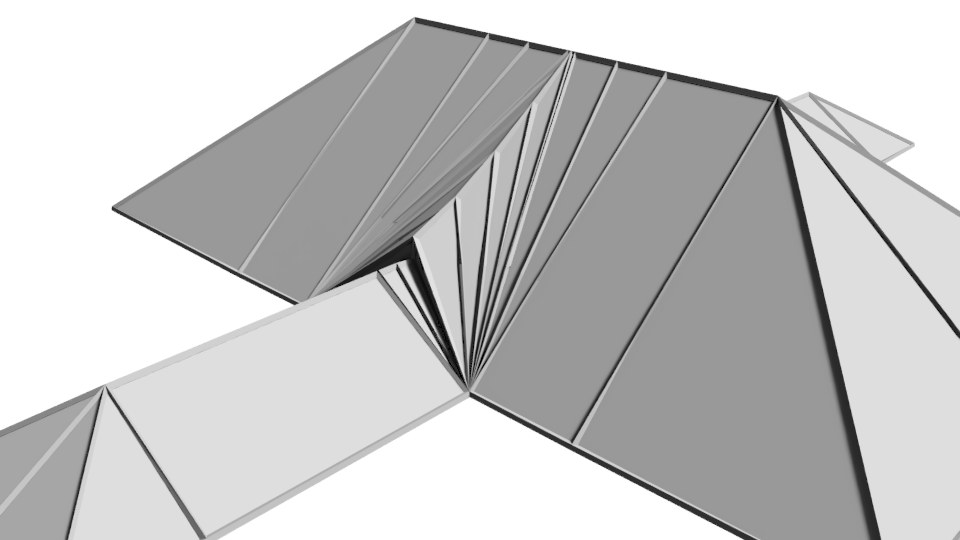
\includegraphics[width=\columnwidth]{sources/method/beading_conflict_3D.png}
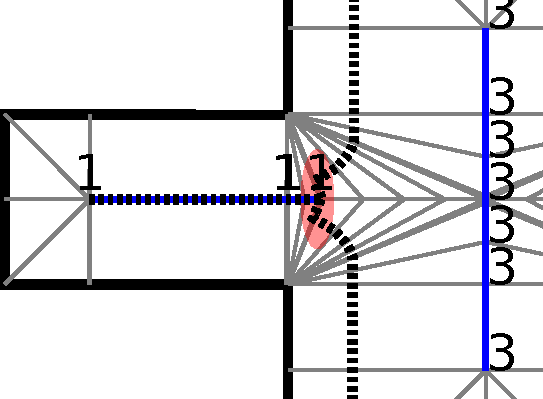
\includegraphics[height=\figheight]{sources/method/beading_conflict.pdf}
\caption{Beading conflict}\label{beading_conflict}
\end{subfigure}
\begin{subfigure}{.45\columnwidth}\centering
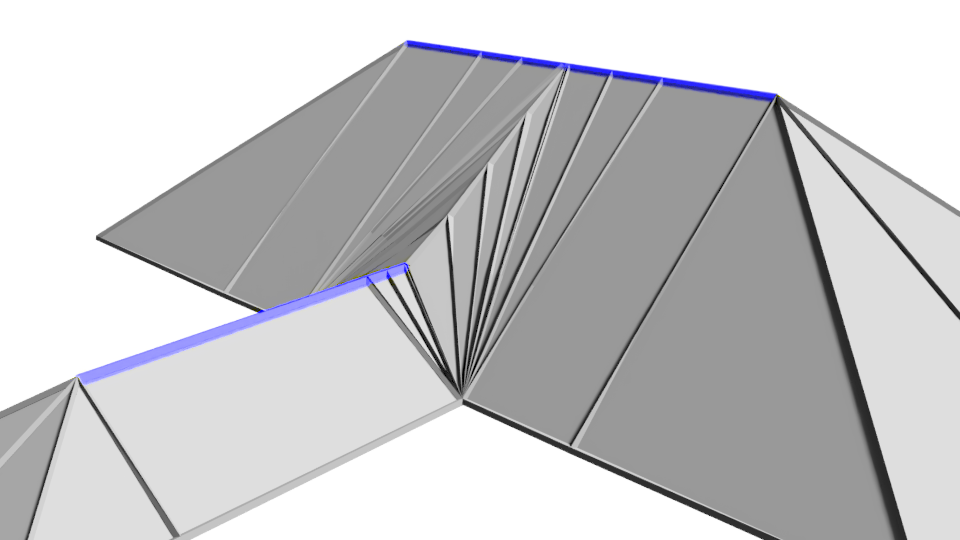
\includegraphics[width=\columnwidth]{sources/method/beading_conflict_solved_3D.png}
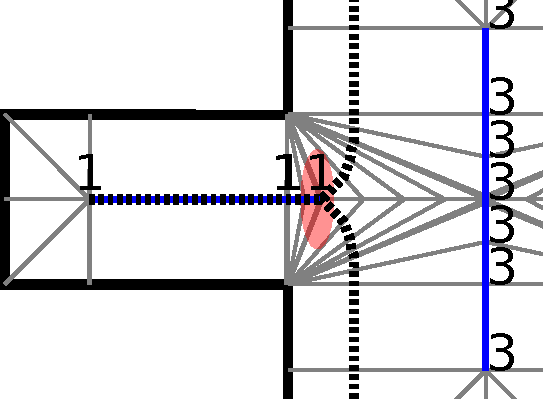
\includegraphics[height=\figheight]{sources/method/beading_conflict_solved.pdf}
\caption{Conflict resolution}\label{beading_conflict_solved}
\end{subfigure}
\caption{
\subref{beading_conflict} The beading propagated from above conflicts with the beading below.
\subref{beading_conflict_solved} The beading conflict is resolved by gradually interpolating between the two beadings.
The ramp to the upper ridge doesn't line up with the lower ridge, which means that
the toolpaths (dashed) resulting from the beading propagated from above doesn't align with the beading from the thin outline feature (highlighted in red).
}
\label{beading_conflict_problem}
\end{figure}


\iffalse

After each marked node is assigned a beading by the beading scheme, we propagate the beadings outward to all nodes in the ST.
The beading propagation is performed in two stages: an upward and downward stage.
%First we sort all upward half-edges on the radial distance of their destination node, so that we can efficiently flood fill the beading information.
In the upward phase we walk from each marked node upward along unmarked edges and map each node encountered to a pair consisting of the traversed distance and the bottom source beading.
In the downward phase we walk from each marked node downward along unmarked edges and map each node to a pair consisting of the traversed distance and the upper source beading -
however, if we encounter a node which was already mapped to an upward propagated beading we employ the interpolation scheme described above in order to define the beading, which is then further propagated downward.
This is implemented in a flood-fill fashion: see \cref{alg_beading_propagation}.

\jun{It is more logical to first explain the general case (the above paragraph), and then the special treatment -- beading conflict.}

\begin{algorithm}
\caption{Beading propagation}
\label{alg_beading_propagation}
\begin{algorithmic}
\ForAll{$v \in$ nodes}
	\If {marked($v$)} $\text{map}[v] = (0, B(b^\wedge_v, 2 R(v)))$ \EndIf
\EndFor
\ForAll{$e \in$ edges}
	\If {$R(v_0^e) < R(v_1^e)$}
		% \State 
		upwardEdges.add($e$)
	\EndIf
\EndFor
\State upwardEdges.sort($\uplambda e_1 e_2 . R(v_1^{e_1}) < R(v_1^{e_2})$) \Comment {low to high $v_1$}
\ForAll{$e \in$ upwardEdges} \Comment{upward phase}
	\If {$\text{map}[v_0^e] \land \neg \text{map}[v_1^e$]}
    		\State $(d, B) = \text{map}[v_0^e]$
    		\State $\text{map}[v_1^e] \leftarrow (d + |v_1^e - v_0^e|, B)$
	\EndIf
\EndFor
\ForAll{$e \in$ reverse(upwardEdges)} \Comment{downward phase}
	\If {$\text{map}[v_1^e]$}
    		\State $(d, B) \leftarrow \text{map}[v_1^e]$
    		% d + |v_1^e - v_0^e|
    		\If {$\text{map}[v_0^e]$}
    			\State $(d_0, B_0) = \text{map}[v_0^e]$
    			\State $B \leftarrow \text{interpolate}(\min(1, d_0 /  t_\text{beading}), B_0, B)$
    		\EndIf
    		\State $\text{map}[v_1^e] \leftarrow (0, B)$
	\EndIf
\EndFor
\end{algorithmic}
\end{algorithm}












\fi



\subsection{Toolpath extraction}\label{sec_toolpath_extraction}
Now that each node has a beading associated with it we can apply the beading to generate the sites of the toolpaths.
For each upward half-edge $e$ we generate each site $J$ based on the beading $B = B^{v_1^e}$:
\begin{align*}
J &= \{ v, w, i \} \\ 
v &= v_1^e + (v_0^e - v_1^e) \frac{R(v_1^e) - l_i^B}{R(v_1^e) - R(v_0^e)} \\ 
w &= w_i^B
% \\ i^J &= i
\end{align*}
for any $i$ for which $R(v_0^e) < l_i^B \leq R(v_1^e)$.
See \cref{site_placement}.
We store all sites of an edge in a mapping from edge to a list of sites.


\begin{figure}
\centering
\setlength{\figheight}{.29\columnwidth}
\begin{subfigure}{0.14\columnwidth}\centering
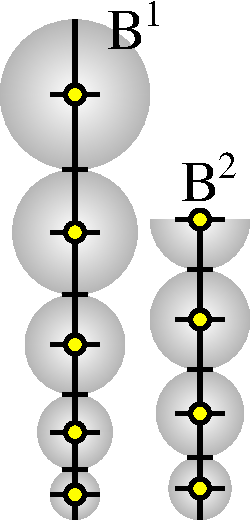
\includegraphics[height=\figheight]{sources/method/trapezoid_beading_beading.pdf}
\caption{Beadings}\label{trapezoid_beading_beading}
\end{subfigure}
\begin{subfigure}{0.5\columnwidth}\centering
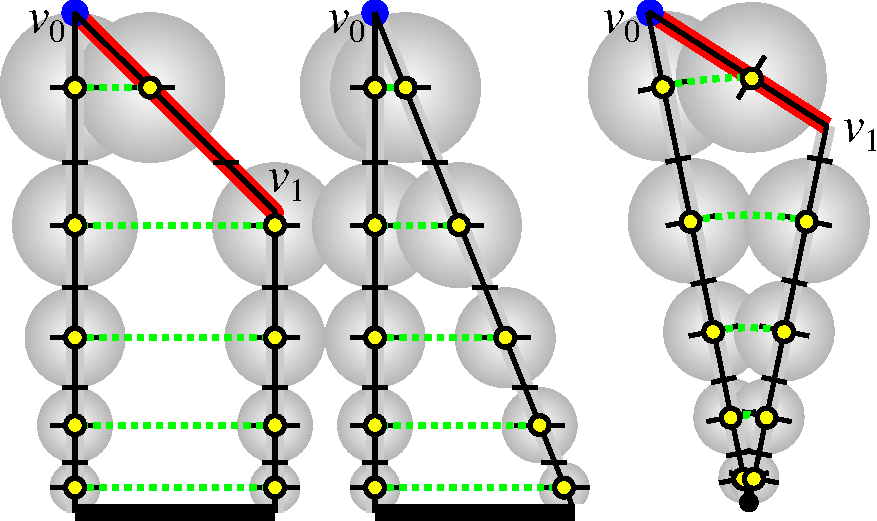
\includegraphics[height=\figheight]{sources/method/trapezoid_beading_propagated.pdf}
\caption{Single beading propagated to all nodes}\label{trapezoid_beading_propagated}
\end{subfigure}
\begin{subfigure}{0.34\columnwidth}\centering
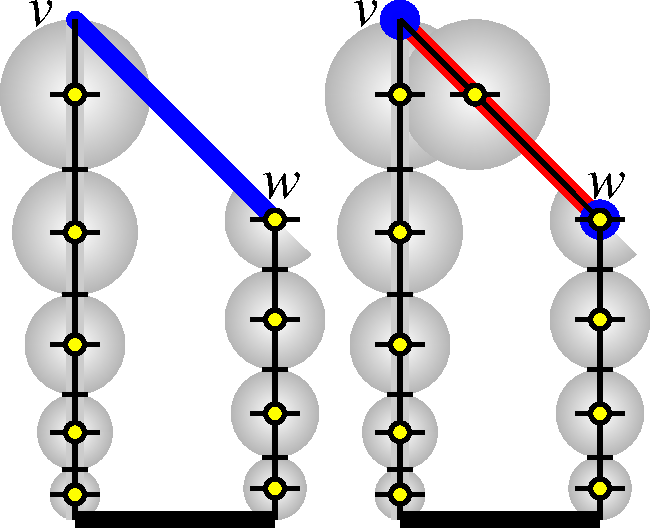
\includegraphics[height=\figheight]{sources/method/trapezoid_beading_separate.pdf}
\caption{Separate beadings at either top node}\label{trapezoid_beading_separate}
\end{subfigure}
\caption{
Applying beadings to generate sites along trapezoids.
\subref{trapezoid_beading_beading} shows half of the locations $l_i$ and widths $w_i$ of two arbitrary different beadings.
\subref{trapezoid_beading_propagated} shows the application of $B^1$ to the various types of trapezoid.
\subref{trapezoid_beading_separate} shows how a trapezoid with a marked edge will have two different beadings assigned, which will generate their respective sites along the support edges.
No sites will be generated along marked edges.
Wide black lines are outline segments, marked nodes and edges in blue, the sites in yellow and green wavefronts of equidistant radial distance at $R = l_i$.
}
\label{site_placement}
\end{figure}


We then generate extrusion segments for each trapezoid by connecting together the sites of the same index.
See \cref{segment_generation}.
If the amount of sites on both sides of the trapezoid is not the same then this trapezoid is in a transition and we leave one inner site unconnected.

Because the bead count is defined in terms of the feature diameter rather than the radius, only some of the bead count values $b^\wedge$ in a central region coincide with a slicing height.
When the bead count $b^\wedge$ is even, the ridge will be sliced as normal;
the intersection between a slicing plane and the mesh surface results in a polyline on both sides of the ridge, which are connected together into a polygonal toolpath.
When the bead count $b^\wedge$ is odd, the ridge will coincide exactly with a slicing height, which results in a single polyline toolpath being generated along the middle of the feature.
In that case we should prevent the algorithm from generating the center extrusion segment twice from the trapezoids on either side of that segment.
We therefore use some arbitrary condition to decide which one of the two to include based on the ordering of the coordinates of $v_0$ and $v_1$: $x_0 < x_1 \lor (x_0 = x_1 \land y_0 < y_1)$.

\tim{Below is taken from an outdated paragraph in section 3.3 (?)}
The trapezoids are classified as belonging to a specific domain following \citeauthor{Ding2016a}.
Each polygon in the input shape acquires it's own domain.
The domains of hole polygons are touching the domains of the outer polygon.
See \cref{shape_decomposition_domains}.

Each of the trapezoids is connecting to a single outline polygon.
By traversing the trapezoids in the domain of each outline polygon in order we can efficiently connect all segments into polylines.
See \cref{segment_generation}.
In a final step we connect the ends of polylines together, so that the final toolpaths contain both polygons and polylines.

\begin{figure}
\centering
\setlength{\figheight}{.3\columnwidth}
\begin{subfigure}{.3\columnwidth}\centering
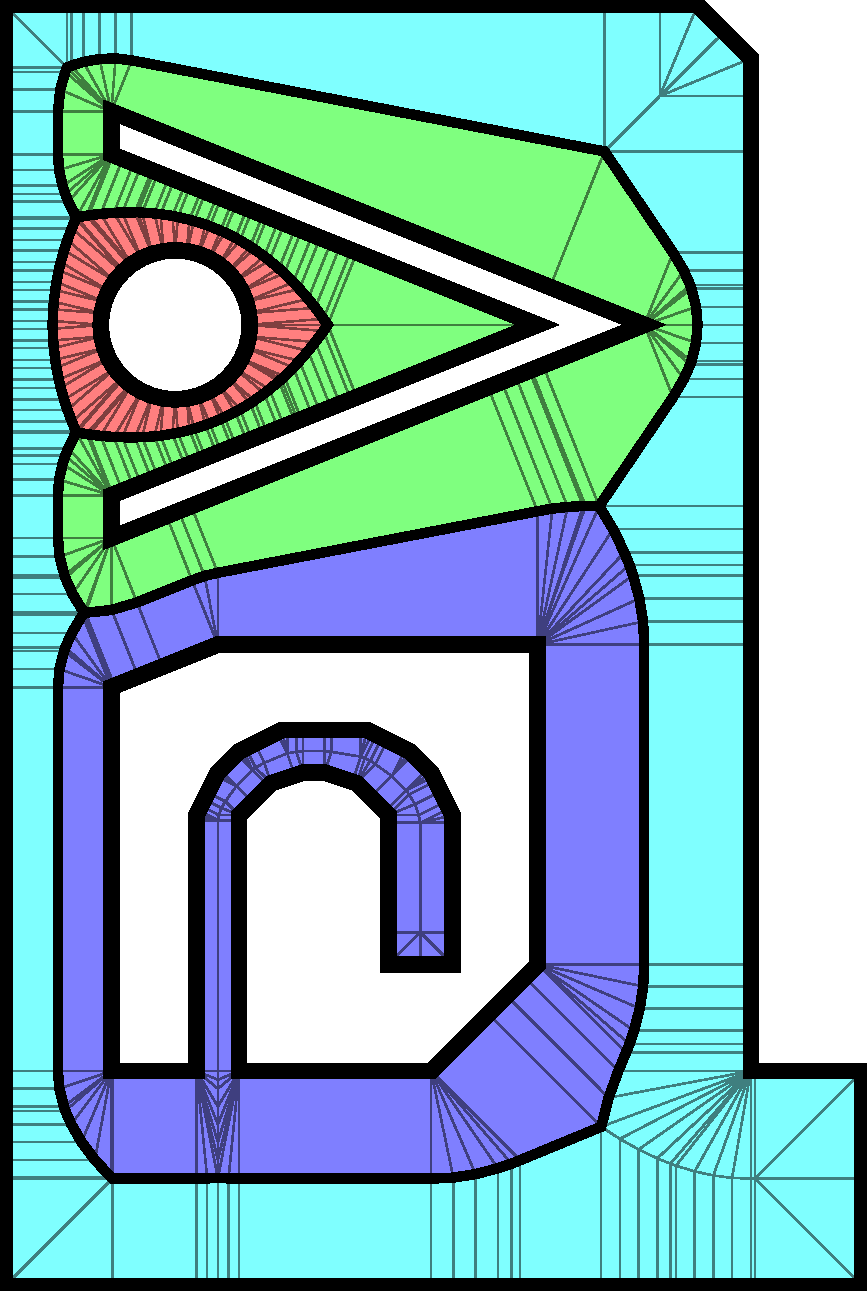
\includegraphics[height=\figheight]{sources/method/domains.pdf}
\caption{Polygon domains}\label{shape_decomposition_domains}
\end{subfigure}
\begin{subfigure}{.6\columnwidth}\centering
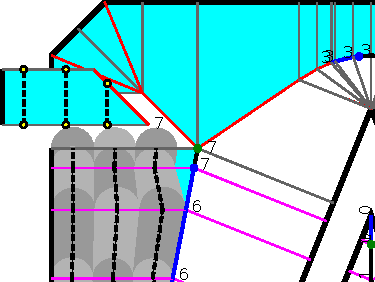
\includegraphics[height=\figheight]{sources/method/segment_generation.pdf}
\caption{Extrusion segment chaining}\label{shape_decomposition_domains}
\end{subfigure}
\caption{
Generating toolpaths on a part of the test outline shape by chaining together extrusion segments along each polygon domain.
Each edge is assigned toolpath sites (yellow) which are connected together as shown in the singled out trapezoid.
By following the trapezoids along the domain (cyan) of a single outline polygon,
the extrusion segments can efficiently be connected into existing polyline toolpaths (light and dark gray).
}
\label{segment_generation}
\end{figure}


Around the transition locations and around nodes with odd bead count and more than two marked edges attached there will be intersections in the toolpaths.
Such intersections cause overfill because the nozzle passes the location multiple times.
We deal with this special case by forcing a new polyline when traversing the trapezoids, and in the final polyline connection step we greadily connect the first two polylines ending in the same location and retreat all other polylines ending in that same location in order to prevent the overfill.
In order to retreat a polyline which ends in a site $J$ we remove part of the polyline paths up to the intersection by a distance of $w^J d_\text{max}^\text{intersection}$, where $d_\text{max}^\text{intersection}$ is some ration between $0$ and $1$.
This ratio effectively deals with the balance between overfill and underfill generated at that location after the retreat has been applied.
See \cref{polyline_reduction}.


\begin{figure}
\centering
\setlength{\figwidth}{.35\columnwidth}
\begin{subfigure}{0.45\columnwidth}\centering
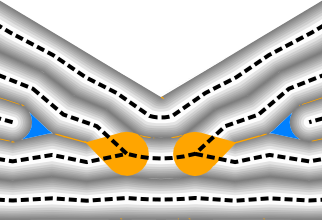
\includegraphics[width=\figwidth]{sources/method/polyline_reduction_before}
\caption{No reduction}
\end{subfigure}
\begin{subfigure}{0.45\columnwidth}\centering
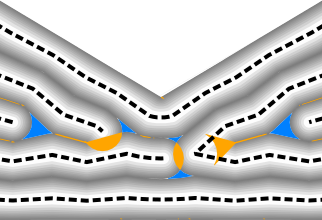
\includegraphics[width=\figwidth]{sources/method/polyline_reduction_after}
\caption{Reduction}
\end{subfigure}
\caption{
Reducing polyline toolpaths away from intersections in order to prevent overfill.
Toolpath locations in black, underfill in azure and overfill in orange.
}
\label{polyline_reduction}
\end{figure}



























































